\documentclass[11pt]{article}

%\usepackage{fontspec}
%\defaultfontfeatures{Mapping=tex-text}
%\setmainfont[BoldFont={Minion Pro Bold}]{Minion Pro}
\usepackage{pdfpages}
%\usepackage[usenames,dvipsnames]{color}
\usepackage{graphicx}
\usepackage{fullpage}

\usepackage{hyperref}

\begin{document}

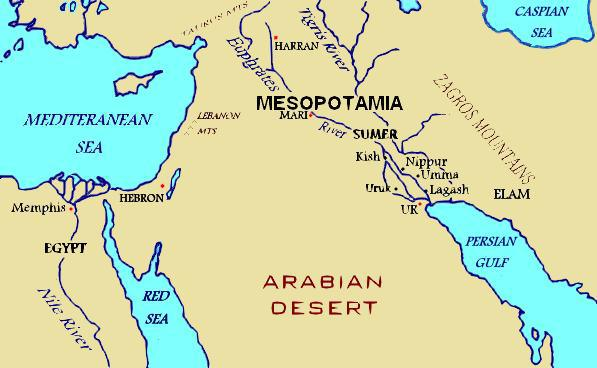
\includegraphics{sumeria.jpg}


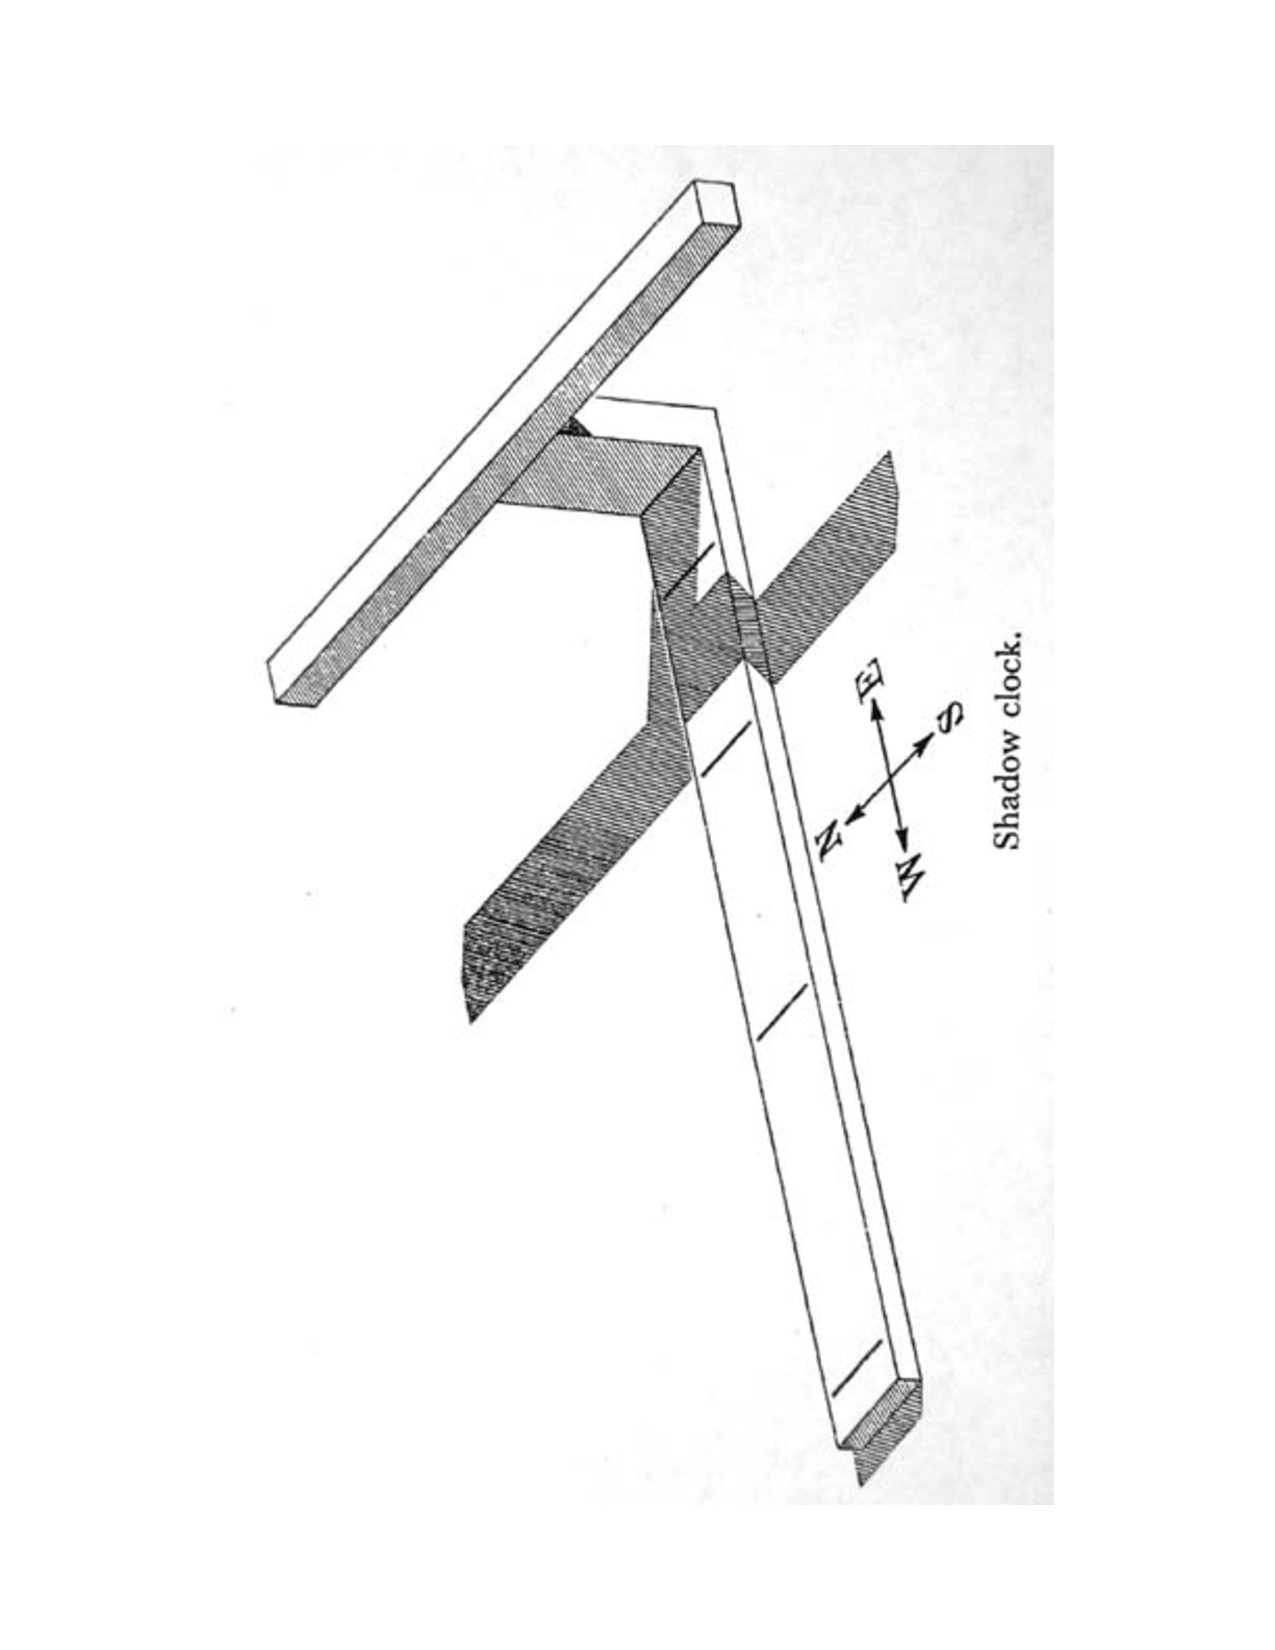
\includepdf{shadow.pdf}


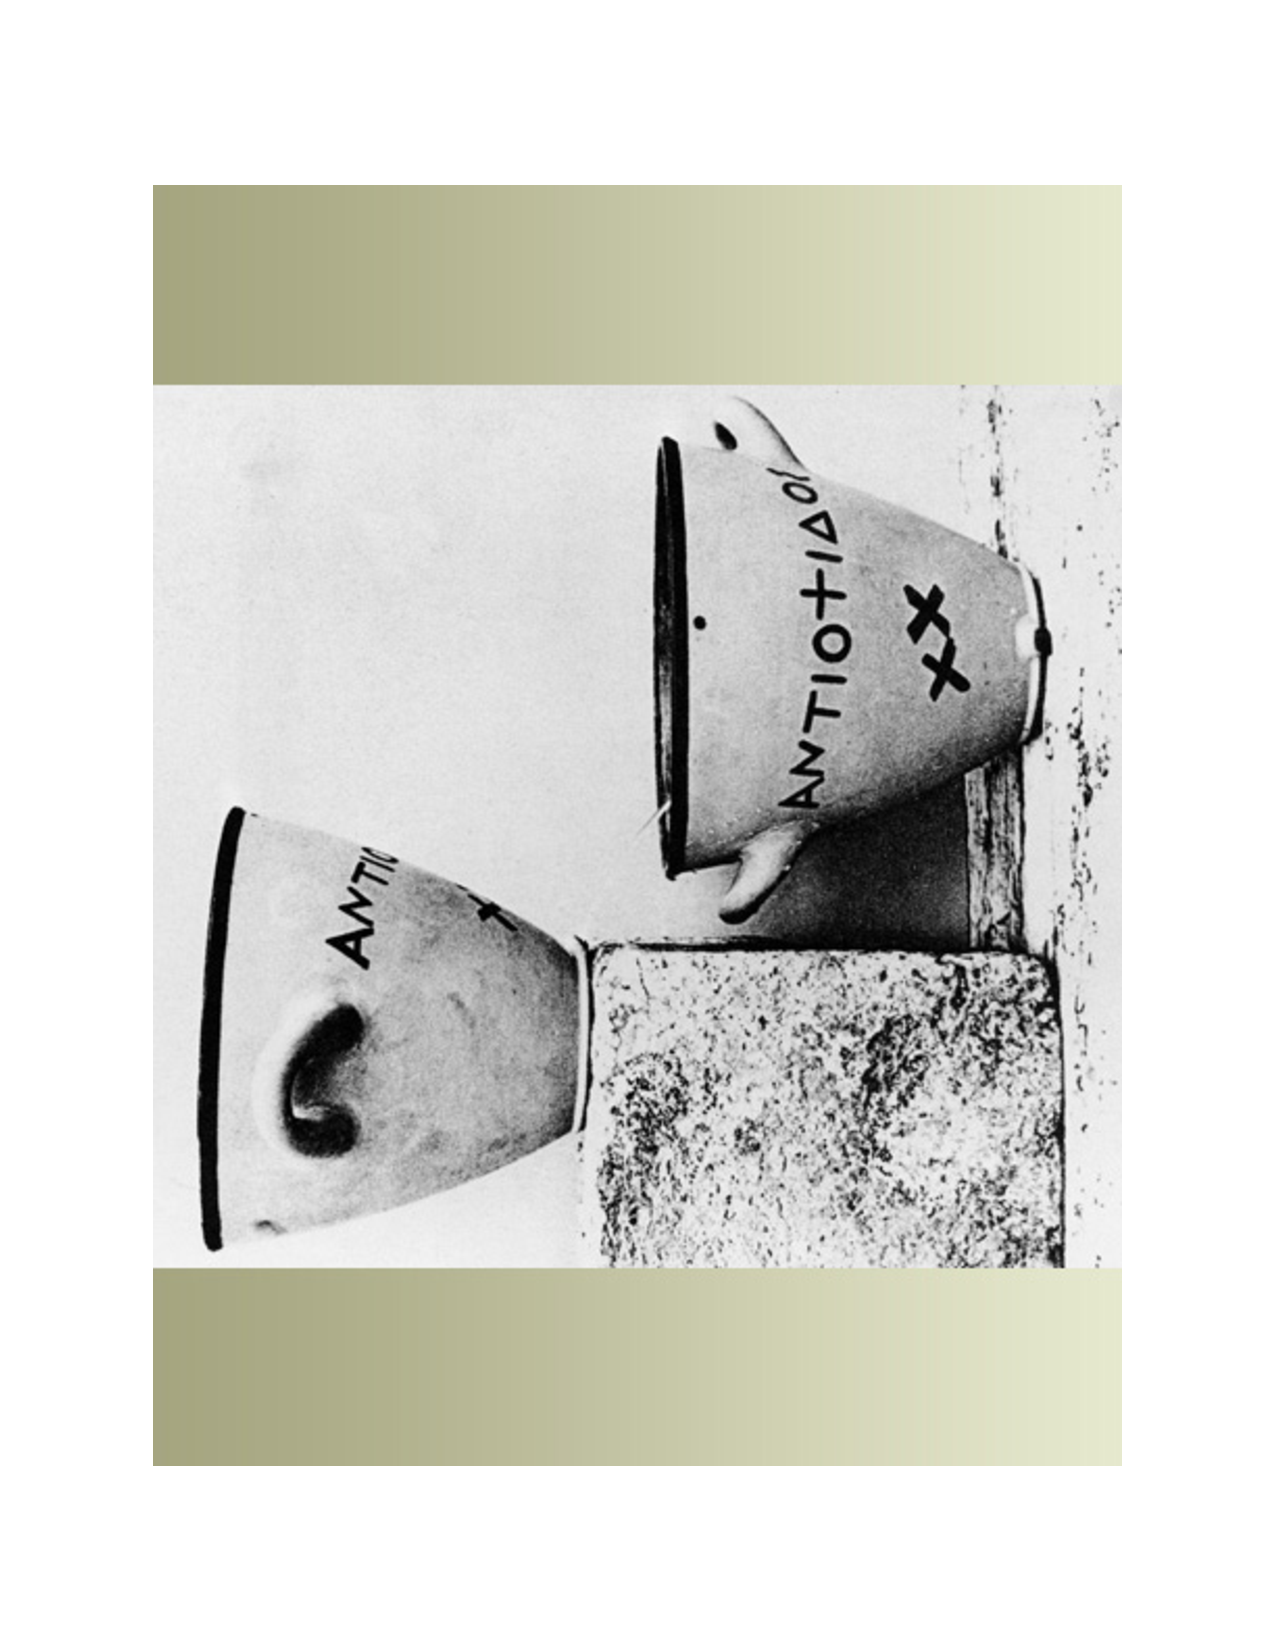
\includepdf{water.pdf}

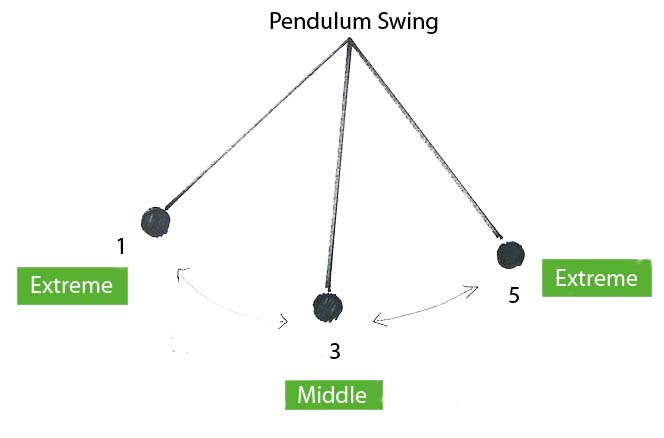
\includegraphics{pendulum.png}

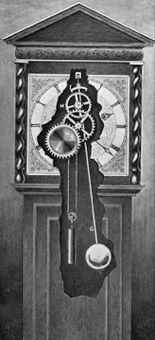
\includegraphics{pendulumclock.jpg}

\newpage
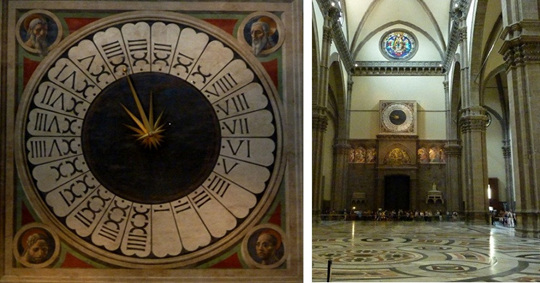
\includegraphics{one.jpg}
\newpage
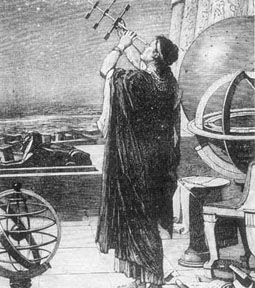
\includegraphics{hipparchus.jpg}

\newpage
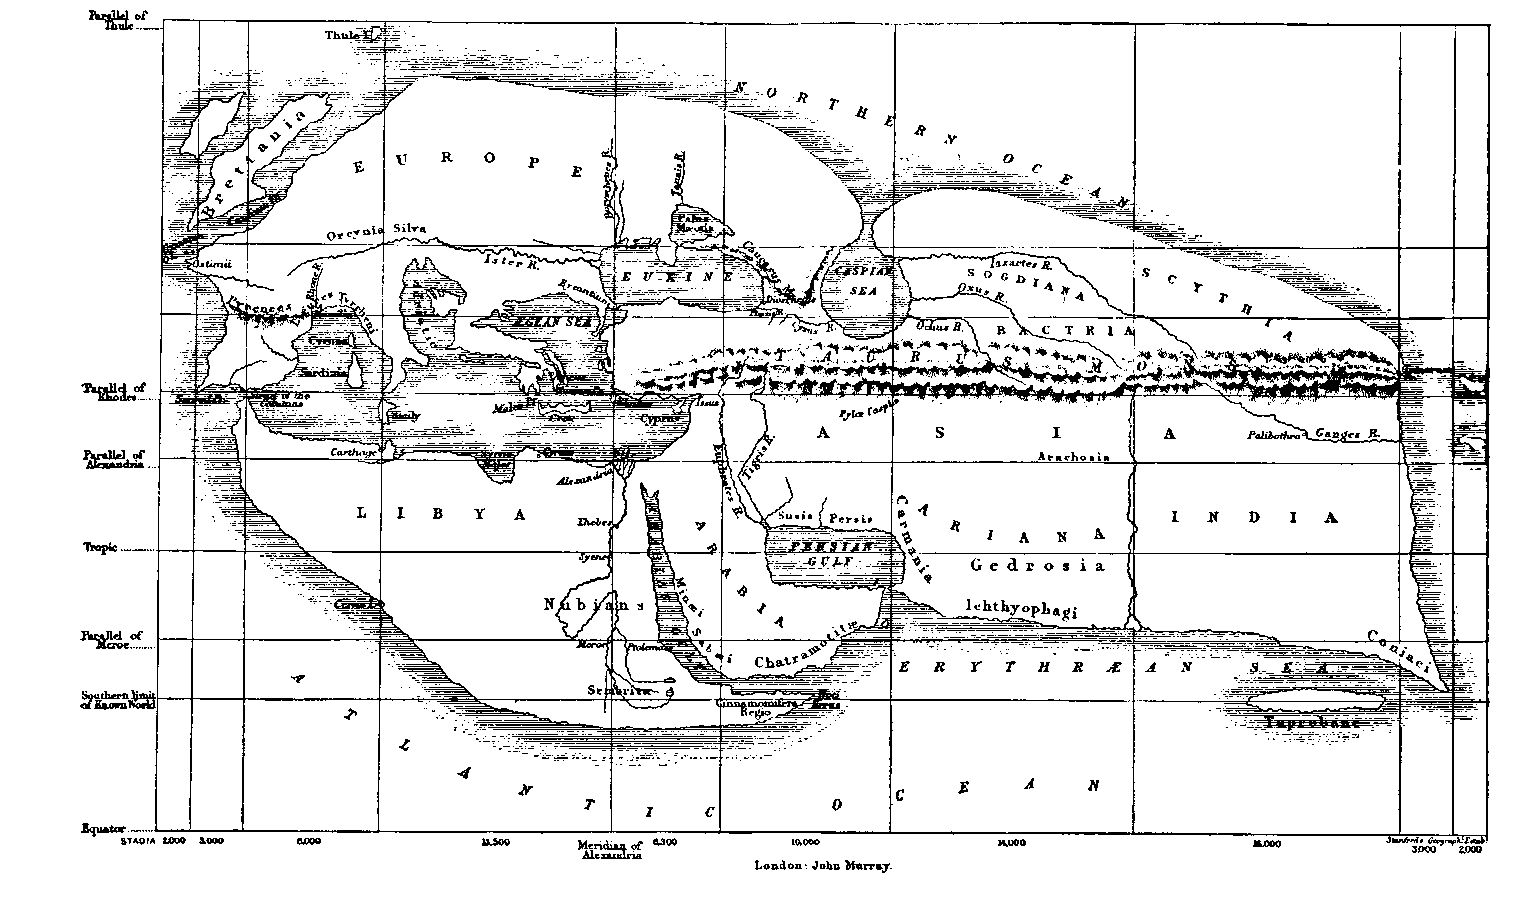
\includegraphics{map.png}
\newpage
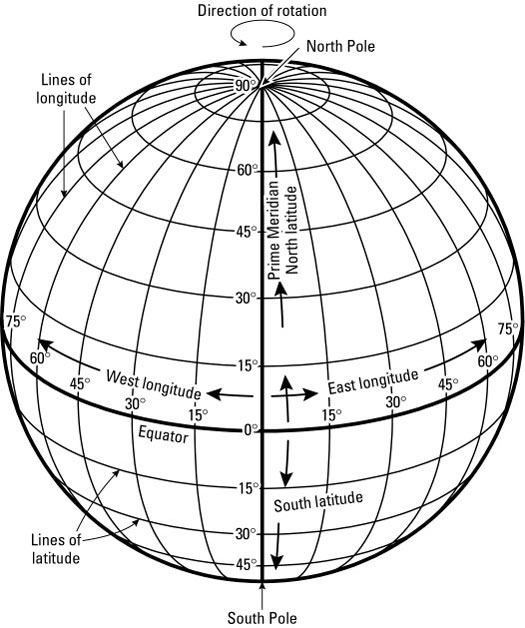
\includegraphics{long.jpg}


\newpage

\section*{Taylorism}

\begin{quote}
 A time chart from the Systems and Procedures
Association of America, for example, suggests target times for activities
like these: open and close file drawer, no selection = .04
seconds; desk, open center drawer = .026 seconds; close center
drawer = .027 seconds; close side drawer = .015 seconds; get up
from chair = .033 seconds; sit down in chair = .033 seconds; turn
in swivel chair = .009 seconds; move in chair to adjoining desk or
file (4 ft. max.) = .050 seconds.(Levin, 'The Geography of Time', p.71)
\end{quote}

\newpage


\section*{Objections}
These are taken from 'A Geography of Time', p.73: 
\begin{itemize}
\item The New York Herald in 1883 observed that
standard time ``goes beyond the public pursuits of men and enters
into their private lives as part of themselves.''
\item ``Let us keep our own noon,'' demanded the prestigious Boston Evening Transcript. 
\item The Louisville Courier Journal referred to standardization as ``a monstrous fraud,'' ``a compulsory
lie,'' and ``a swindle.''
\item  A letter to that newspaper asked, ``if anyone has the authority
and right to change the city time without the consent of
the people, and what benefit Louisville can derive from it?''
\item The editors responded that no such authority ruled, and no
benefit seemed likely from what was ``only a disguised step
towards centralization ...a stab in the dark at our cherished
State's rights. 
\item After they get all our watches and clocks ticking
together,'' the editors asked in reflexive alarm, ``will
there not be a further move to merge the zone states into
districts or provinces?'
\end{itemize}

\newpage


\section*{Is Time a fictional master?}
\
\begin{quote}
When I was alive, I believed---as you do---that time was at
least as real and solid as myself, and probably more so. I said
``one o'clock'' as though I could see it, and ``Monday'' as though I could find it on a map ... Like everyone else, I
lived in a house bricked up with seconds and minutes, weekends
and New Year’s Days, and I never went outside until I
died, because there was no other door. Now I know that I
could have walked through the walls. (Peter Beagle, 'The Last Unicorn')
\end{quote}






\end{document}
